\chapter{Capacidade de Acomodação de Recursos Energéticos Distribuídos}

Neste capítulo, são apresentados os principais conceitos e aspectos de \ac{HC}. Inicialmente é apresentado brevemente o contexto em que este conceito se aplica em sistemas de distribuição, na qual a presença de geradores distribuídos já é uma realidade e há uma perspectiva de aumento nos anos seguintes. Em seguida, este contexto é confrontado com a dificuldade de se mensurar a capacidade que sistemas de distribuição têm de acomodar novos geradores distribuídos e como este problema se relaciona com o \ac{PESD}. Desta forma, são apresentadas as principais abordagens encontradas na literatura para identificar, mensurar e melhorar o valor de \ac{HC}, bem como as considerações realizadas para tal. Por fim, é apresentada a proposta de integração de um indicador de \ac{HC} no modelo de \ac{PESD} abordado no capítulo anterior.

Esta proposta é baseada no espelhamento das restrições de comportamento do sistema de distribuição do modelo base, no qual cria-se novas variáveis para as tensões nodais, fluxo de corrente nos ramos e injeção de corrente dos transformadores e geradores distribuídos. A partir deste espalhamento cada nó recebe a nova variável que representa a injeção de corrente de futuros recursos energéticos distribuídos. Por fim, é adicionado na função objetivo base um novo parâmetro que busca maximizar o valor da soma destas novas injeções. Desta forma, e no mesmo modelo, é possível avaliar tanto o custo com o \ac{PESD}, quanto o \ac{HC} de cada nó e do sistema por inteiro. Por outro lado, algumas limitações podem ser observadas no modelo de modo que uma análise numérica destas limitações se torna necessária. Esta análise é realizada no próximo capítulo deste trabalho, porém, alguns levantamentos e possíveis problemas já são abordados neste. 

Ao final deste capítulo, espera-se que o contexto atual em que os sistemas de distribuição se encontram e a problemática relacionada à grande presença de geradores distribuídos esteja clara, bem como a proposta de integração do problema de \ac{PESD} e da métrica adotada para o \ac{HC}.


\section{Conceitos sobre a capacidade de acomodação}


O problema da integração de recursos energéticos distribuídos em sistemas de distribuição vem sendo discutido desde o surgimento destes geradores. Atualmente, observa-se que há uma tendência de tornar o sistema de distribuição mais controlável, principalmente devido aos problemas causados pelas intermitências das fontes renováveis destes geradores. Esta tendência se traduz no conceito de \textit{smart grid} que pode ser definido como um sistema altamente observável por meio de medições e controlável remotamente (incluindo de forma autônoma) através dos mais diversos dispositivos instalados. Por outro lado,  segundo \citeonline{Tuballa2016710}, observa-se que muitas tecnologias relacionadas ao conceito de \textit{smart grid} ainda estão em fase de pesquisa e desenvolvimento e, principalmente em países em desenvolvimento, este conceito pode levar alguns anos (até décadas) para ser amplamente adotado. 

Neste contexto de transição, surge o conceito de capacidade de acomodação de recursos energéticos distribuídos (\ac{HC}), no qual é um indicador de alta abstração do sistema de distribuição que demonstra a quantidade e potência máxima de recursos energéticos distribuídos que podem ser instalados. Ao utilizar este indicador, os engenheiros de planejamento da empresa distribuidora e outros investidores podem avaliar a disponibilidade de novos investimentos sem a necessidade de grandes alterações no sistema de distribuição, tornando estas tomadas de decisões mais claras e objetivas.

Além de avaliar o indicador, também é possível realizar alterações no sistema de distribuição com o objetivo de melhorar este indicador. Estas alterações podem fazer parte do plano de \ac{PESD}, alterando a topologia do sistema, alocação de novos dispositivos ou alterações da proteção do sistema de distribuição. Por outro lado, a melhoria do indicador também pode fazer parte da operação, utilizando chaves para alterações topológicas, chaveamento de banco de capacitores, controlando geradores distribuídos despacháveis ou sistemas de armazenamento de energia. Desta forma, pode-se afirmar que qualquer alteração no sistema de distribuição pode melhorar ou piorar o indicador de \ac{HC}, seja de uma forma temporária, durante a operação, ou permanente através do \ac{PESD}.

De modo geral, a figura \ref{fig:hc} demonstra a curva de desempenho de um sistema de distribuição com e sem melhoria do \ac{HC}. Pode-se observar que até certo valor de penetração de recursos energéticos distribuídos o sistema de distribuição possui uma operação aceitável, porém com o aumento da penetração a operação do sistema passa a não ser aceitável, violando algum limite operacional ou de equipamentos. 


\begin{figure}[ht]
 	\centering
    \caption{Curva de desempenho de um sistema de distribuição em relação à penetração de geradores distribuídos e sua capacidade de acomodação antes e depois de uma melhoria.}
    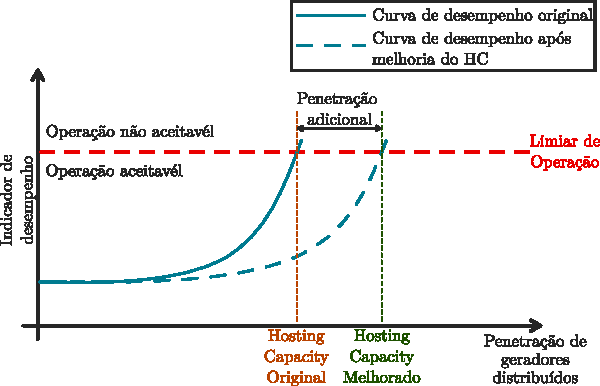
\includegraphics[width=0.8\textwidth]{cap3/HC.pdf}\\
    Fonte: Adaptado de \citeonline{HCStateArt}
    \label{fig:hc}
\end{figure}

A forma de obter o valor de \ac{HC} varia de acordo com a metodologia adotada. Para \citeonline{smith2012stochastic}, em seu relatório para o Electric Power Research Institute, o \ac{HC} pode ser definido através de violação de tensão, carregamento de linhas, dispositivos de proteção, qualidade de energia e controle. Já para \citeonline{palmintier2016path}, em seu relatório para o Departamento de Energia dos Estados Unidos, o \ac{HC} é a capacidade de instalação de novos recursos energéticos distribuídos de um sistema de distribuição sem alteração topológica, instalação de novos dispositivos ou recondutoramento. 


De qualquer forma, podemos definir duas classes de \ac{HC}, o global e o local. O \ac{HC} local é capacidade máxima que uma região ou barramento do sistema possui de instalação de novos recursos energéticos distribuídos. O \ac{HC} global é capacidade máxima que um sistema de distribuição, como um todo, possui de instalação de novos recursos energéticos distribuídos. 
Estes novos recursos energéticos distribuídos, geralmente buscam obter alguma vantagem financeira, seja por serviços ancilares para o sistema de distribuição, seja por redução dos custos com energia elétrica de outras empresas, há também a utilização para arbitragem, porém, geralmente sistemas de armazenamento de energia são mais recomendados nesta operação.
No Brasil, os serviços ancilares ainda não são regulamentados e, portanto, os novos recursos energéticos distribuídos, geralmente buscam redução de custos com energia elétrica ou venda de energia em mercados livres.
Desta forma, o termo \ac{HC} vem sendo amplamente utilizado como forma de indicar quanto um sistema de distribuição pode hospedar recursos energéticos distribuídos não ancilares.

Este crescimento na penetração de recursos energéticos distribuídos não ancilares, vem se tornando uma das principais preocupações das empresas distribuidoras, visto que a presença desses geradores causam diversas perturbações na qualidade de energia, operação e segurança do sistema de distribuição. Segundo o trabalho de \citeonline{HCStateArt}, estima-se um aumento de 58\% nos custos da operação dos sistemas, sendo que 55\% deles atingirão seus limites operacionais nos próximos 10 anos, caso esse crescimento de recursos energéticos distribuídos se mantenha.

Vale salientar que  a empresa distribuidora raramente pode prever a futura existência de recursos energéticos distribuídos de outras empresas em seu sistema de distribuição durante a fase de planejamento. Porém, é de grande importância que a empresa distribuidora possua uma estimativa do valor de \ac{HC} do seu sistema durante esta fase, pois, este indicador ajuda a demonstrar a viabilidade de novos investimentos de outras empresas em seu sistema de distribuição. 

Dentro deste contexto, as empresas distribuidoras vêm realizando diversos esforços para mensurar e para melhorar o valor de HC de seus sistemas de distribuição. E estes esforços se traduzem também nos trabalhos acadêmicos que têm demonstrado interesse neste tema, como será apresentado a seguir.

\section{Capacidade de acomodação na literatura acadêmica}

Segundo \citeonline{en10091325}, o conceito de HC foi inicialmente cunhado por André Even em Março de 2004 durante discussões no projeto EU-DEEP project. Em artigos acadêmicos, este conceito é primeiramente encontrado em \citeonline{Bollen2005} ao descrever os problemas de qualidade de energia relacionados à inserção de recursos energéticos distribuídos em sistemas de distribuição. Segundo \citeonline{Bollen2005} o cálculo de HC deve ser realizado para diversos fenômenos da operação e planejamento e que este valor não é fixo e depende também da estrutura do sistema de distribuição. Neste mesmo artigo o autor apresenta que há um possível \textit{trade-off} entre os custos de investimento no sistema de distribuição e a melhoria do valor de HC. Apesar desta afirmação, o autor se ateve aos problemas de qualidade da energia, descrevendo algumas formas de calcular o HC para os problemas de qualidade da tensão e de harmônicas.

Entretanto, o termo HC e sua análise só obteve adesão considerável por parte da literatura acadêmica a partir de 2014. Um indicador desta adesão pode ser vista na figura \ref{fig:scopus} que demonstra o número de artigos em revistas científicas indexados no sistema Scopus da Elsevier (um dos maiores indexadores de trabalhos acadêmicos do mundo) durante o período de 2005 a 2020 utilizando a query:

\vspace{-1pt}
\noindent\textit{TITLE-ABS-KEY ( "Hosting Capacity" )  AND  PUBYEAR  >  2004  AND  PUBYEAR  <  2021  AND  ( LIMIT-TO ( SUBJAREA ,  "ENGI" )  OR  LIMIT-TO ( SUBJAREA ,  "ENER" ) )  AND  ( LIMIT-TO ( DOCTYPE ,  "ar" ) )}


\begin{figure}[ht]
 	\centering
    \caption{Quantidade de artigos indexados no sistema Scopus da Elsevier durante o período de 2006 a 2020 (entre 2005 e 2009 não houve artigos).}
    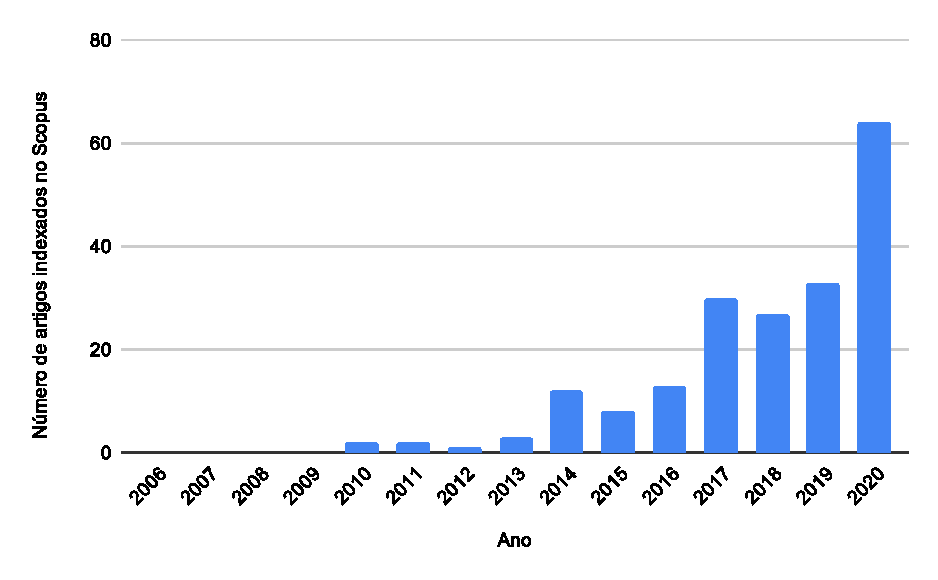
\includegraphics[width=0.8\textwidth]{cap3/chart.pdf}\\
    Fonte: Adaptado de \citeonline{scopus}
    \label{fig:scopus}
\end{figure}

Uma tese sobre esta adesão tardia ocorreu devido ao consenso acadêmico anterior de que a empresa distribuidora teria um grande poder de decisão relacionado a localização, potência instalada e operação de recursos energéticos distribuídos no sistema de distribuição. Este consenso acadêmico da época levou diversos trabalhos acadêmicos até os dias atuais a considerarem que a empresa distribuidora pode decidir o melhor planejamento destes geradores. Curiosamente, uma síntese do estado da arte destes tipos de trabalhos foi publicada por \citeonline{6307952} um ano antes de uma maior adesão acadêmica do termo HC. Atualmente, pode-se afirmar que a empresa distribuidora atua muito mais como um limitador da quantidade e potência de recursos energéticos distribuídos no sistema de distribuição do que um operador destes geradores, com exceção dos geradores com objetivos ancilares.


Outra hipótese sobre esta adesão ter ocorrido a partir de 2014 foi o crescimento de recursos energéticos distribuídos de fontes renováveis em sistemas de distribuição da Europa desde 2004, causados pelos incentivos fiscais e financeiros realizados na \citeonline{eurotstat}.

Nesta revisão da literatura, apenas os trabalhos que lidam diretamente com \ac{HC} foram incluídos, visto que, com a popularização do termo, muitos trabalhos apresentam a melhoria do \ac{HC} como um efeito secundário em relação ao real objetivo do trabalho. Dentre os trabalhos que abordam o conceito de \ac{HC}, podemos dividir estes trabalhos nos seguintes tópicos abaixo que serão explicados a seguir:

\begin{itemize}
    \item formas de mensurar e avaliar a capacidade de acomodação;
    \item medidas de melhoria da capacidade de acomodação por integração do controle da operação dos recursos energéticos distribuídos;
    \item medidas de melhoria da capacidade de acomodação por controle de outros dispositivos no sistema de distribuição.
\end{itemize}
\vfill 

\subsection{Formas de mensurar e avaliar a capacidade de acomodação}

Neste tópico, os trabalhos discutem aspectos sobre quais fatores devem ser considerados ao se avaliar o valor de \ac{HC} de um sistema de distribuição de forma prática, seja durante a operação ou para o planejamento.

Dentre estes trabalhos, está incluso o trabalho de \citeonline{Bollen2005} que discute os como mensurar os impactos de geradores distribuídos na qualidade da energia. Já o trabalho de \citeonline{PAPAIOANNOU2014141} descreve uma metodologia analítica para identificar a melhor localização de um gerador distribuído em um sistema de distribuição de baixa tensão. No trabalho de \citeonline{SANTOS2015199} são descritos os impactos nos componentes harmônicos com o aumento da presença de geradores distribuídos baseados em inversores e propõem uma metodologia para definir o \ac{HC} do sistema de distribuição deste ponto de vista. 

Partindo de um outro ponto de vista, o trabalho de \citeonline{en8031760} descreve o impacto de carregadores de veículos elétricos em sistemas de distribuição de baixa tensão e aplica o conceito de \ac{HC} para este novo tipo de dispositivo no sistema de distribuição. No mesmo tópico de avaliar novos recursos distribuídos, o trabalho de \citeonline{7155600} avalia o comportamento de recursos distribuídos de baixo impacto ambiental em sistemas de distribuição de baixa tensão e indica que as avaliações realizadas podem ser utilizadas na avaliação do  \ac{HC}.

O trabalho de \citeonline{7219464} utilizou a mesma estratégia de analisar o comportamento, só que aplicado a geradores distribuídos, para determinar diversas correlações entre a potência, localização e \ac{HC} em sistemas de distribuição e propor uma metodologia simples para avaliar o \ac{HC} de sistemas de distribuição.

O trabalho de \citeonline{en10091325} realiza uma discussão sobre o conceito de \ac{HC} para o planejamento de sistemas de distribuição, nele uma análise para os piores casos de sobretensão e subtensão é realizada e uma discussão sobre os outros problemas são relacionados aos problemas de tensão discutidos. Por fim, é salientado que dados sobre outros recursos distribuídos são necessários para uma análise mais profunda sobre este conceito.

No trabalho de \citeonline{7723860} avalia-se o caso de geradores distribuídos fotovoltaicos e descreve um modelo para estimar o HC utilizando simulação de Monte Carlo para considerar o comportamento estocástico destes geradores. Utilizando uma estratégia parecida, o trabalho de \citeonline{7913608} propõe a determinação do HC através de risco associado devido às incertezas de geradores distribuídos renováveis. Já no trabalho de \citeonline{8270364} foi desenvolvida a mesma estratégia para verificar os riscos relacionados ao HC de geradores distribuídos fotovoltaicos em 50 mil sistemas de distribuição de baixa tensão e foi identificado um comportamento log-normal no risco de violação dos indicadores de HC.  O trabalho de  \citeonline{7763786} baseia-se nos dados obtidos via simulação de sistemas de distribuição ativos para determinar de forma robusta o valor de HC através de otimização linear.


Por outro lado, o trabalho de \citeonline{8325320} realiza uma linearização do problema de HC para desenvolver um método de avaliação do valor através da proposição de um \textit{framework} probabilístico que considera as incertezas da geração distribuída. Em \citeonline{ALTURKI2018350} é proposto outro modelo linearizado para determinar o valor de HC de um sistema de distribuição, segundo os autores, os resultados são obtidos mais rapidamente porém com um pequeno erro. Já no trabalho de \citeonline{Sousa2020}, uma margem prática de estimar o valor de HC é proposta para sistemas de distribuição de baixa tensão com geradores distribuídos fotovoltaicos com inversores inteligentes.

Analisando veículos elétricos, o trabalho de \citeonline{7817888} descreve o conceito de região "carregável", na qual descreve a quantidade de demanda de carregamento de veículos elétricos que um sistema de distribuição pode acomodar em um determinado momento. Esta análise é realizada através de otimização considerando que a empresa distribuidora pode atrasar um carregamento. 

Já o conceito de HC dinâmico foi melhor desenvolvido no trabalho de \citeonline{en12132576} que descreve que um sistema de distribuição possui três níveis de HC: pior, o médio e o melhor, estes valores variam no tempo e no local de estudo. Para esta avaliação, foi verificado o impacto das distorções harmônicas e variação de tensão causados por geradores distribuídos fotovoltaicos.

\subsection{Medidas de melhoria da capacidade de acomodação por integração do controle da operação dos geradores distribuídos} \label{hc_review_control_dg}

Neste tópico, são descritos os métodos que pressupõem um controle sobre o recurso energético distribuído por parte da empresa distribuidora, seja pela utilização de inversores distribuídos inteligentes ou por contratos com os donos dos geradores.

Dentro deste conceito, podemos elencar o trabalho de \citeonline{CALDERARO201464} que descreve uma estratégia de gerenciamento de geradores distribuídos de fontes renováveis através do controle da potência ativa e reativa evitando que estes geradores sejam desconectados por limites de tensão, em seus resultados é observado que um gerenciamento desses recursos poderiam aumentar a capacidade de acomodação do sistema de distribuição. Na mesma direção, o trabalho de \citeonline{6744682} descreve uma estratégia de gerenciamento ativo para melhorar a capacidade de acomodação de geradores eólicos em sistemas de distribuição através da redução da energia gerada, mudança de taps de reguladores e geração de energia reativa, o autor obteve resultados que demonstravam que um gerenciamento destes geradores e de outros dispositivos no sistema de distribuição podem aumentar a capacidade de acomodação de geradores distribuídos. 

Outra estratégia utilizando gerenciamento ativo do sistema de distribuição é proposta por \citeonline{Quijano2017}, no qual busca minimizar as perdas do sistema de distribuição enquanto maximiza a capacidade de injeção de potência dos geradores distribuídos instalados. Unindo estes controles com a possibilidade de recondutoramento, o trabalho de \citeonline{8678766} já propõe uma avaliação estocástica via simulação de Monte Carlo para melhoria do HC de geradores distribuídos fotovoltaicos. 


O trabalho de \citeonline{7534843} explora os aspectos de planejamento multiestágio da alocação de geradores distribuídos no sistema de distribuição com o objetivo de maximizar o valor de HC. Esse planejamento passa pela coordenação probabilística da operação entre os geradores distribuídos, sistemas de armazenamento de energia e dispositivos de geração de potência reativa, neste trabalho também é observado um modelo de planejamento linear diferente dos modelos propostos no problema do \ac{PESD}. Já no trabalho de \citeonline{RABIEE2017417} é proposta a maximização do HC através da otimização da operação de grandes usinas de geração eólica. O trabalho de \citeonline{en12193610} desenvolve um planejamento integrado entre o sistema de transmissão e o valor esperado de HC de sistemas de distribuição ligados à transmissão.

O trabalho de \citeonline{COLLINS2015464} descreve a eficácia do controle de potência ativa e reativa de geradores distribuídos baseados em inversores para a melhoria do HC do ponto de vista de sobre tensão.  Já \citeonline{HU2016264} descreve uma coordenação entre \acp{OLCT} e inversores de geradores distribuídos fotovoltaicos para o gerenciamento de sistemas de distribuição desbalanceados e descreve em seus resultados que esta coordenação eleva consideravelmente o valor de HC. No trabalho de \citeonline{8046055} é utilizado técnicas de gestão ativa do sistema de distribuição para avaliar um valor robusto de HC através de otimização linear inteira-mista. 

Uma análise da sensibilidade de sistemas de distribuição a geradores distribuídos fotovoltaicos foi realizado no trabalho de \citeonline{7784836}, no qual, também propõem que avaliação do HC passa por um modelo de otimização que define as variáveis de controle de sistemas de distribuição ativas (chaveamento de banco de capacitores, reguladores de tensão, alteração na topologia e controle dos inversores dos geradores).

Um estudo mais aprofundado do impacto da possibilidade de controle dos geradores distribuídos baseados em inversores foi realizado por \citeonline{8895828}. Os resultados apontam para uma melhoria considerável no valor de HC quando há a possibilidade de controle de potência ativa e reativa destes geradores.
\vfill

\subsection{Medidas de melhoria do HC por controle de outros dispositivos no sistema de distribuição}

Nesta seção estão descritos os métodos e trabalhos que propõe a melhoria do HC através apenas do controle de outros dispositivos no sistema de distribuição, seja em um contexto de \textit{smart grids} ou não.


O trabalho de \citeonline{6818426} é um dos primeiros trabalhos que parte do problema clássico de reconfiguração do sistema de distribuição para a melhoria do HC. Este trabalho baseia-se na premissa da existência de chaveamento remoto e é baseado no modelo de fluxo de potência ótimo. O conceito de HC é definido pelos limites de tensão em estado permanente e limites térmicos das linhas de distribuição, os autores salientam que o trabalho está inserido no contexto de planejamento da operação pois o problema exigiu um poder computacional e tempo considerável. Baseado no mesmo problema, \citeonline{8279492} propõe a utilização de um algoritmo de decisão \textit{fuzzy} e métodos meta-heurísticos de otimização para determinar uma boa reconfiguração. Já no trabalho de \citeonline{en13205446}, \textit{soft open points} são adicionados no problema de reconfiguração através de um problema de otimização multiobjetivo que busca minimizar perdas enquanto maximiza o valor de HC.

Já o trabalho de \citeonline{7426863} descreve a utilização de \ac{OLCT} e de compensadores de potência reativa estáticos para avaliar o HC considerando que estes chaveamentos são realizados pela empresa distribuidora durante o planejamento da operação. Seguindo a discussão de utilização de novos dispositivos, o trabalho de \citeonline{LONG2016427} propõe a utilização de \textit{soft open points} para aliviar o carregamento das linhas e problemas com sobretensão e, assim, melhorar o HC. Já o trabalho de \citeonline{7317829} descreve uma estratégia utilizando o \ac{OLCT}, banco de capacitores e um sistema de monitoramento aplicado a sistemas de distribuição de baixa tensão para melhoria do HC. 


Através de mecanismos de resposta da demanda no contexto de \textit{smart grids}, o trabalho de \citeonline{SOROUDI2017316} busca obter um equilíbrio entre as perdas do sistema de distribuição e melhoria do valor de HC, este problema é modelado na forma de otimização bi-objetiva não linear. Já avaliando apenas compensadores de potência reativa estáticos, o trabalho de \citeonline{XU2019952} propõe um planejamento ótimo da alocação e operação desses dispositivos e identifica que há uma melhoria significativa do HC para geradores distribuídos fotovoltaicos. Por outro lado, o trabalho de \citeonline{8481391} já propõe um controle adaptativo destes dispositivos baseando-se no conceito de HC dinâmico. Já um gerenciamento das cargas em sistemas de distribuição de baixa tensão baseado em programação linear é proposto por \citeonline{Bakhtiari2020}, no qual poucos dados compartilhados entre os consumidores e a empresa de distribuição são necessários.

Através de aspectos práticos (como por exemplo, rebalanceamento de cargas nas fases do sistema), o trabalho de \citeonline{Wong2017} propõe diversas medidas que podem ser adotadas antes de necessariamente aplicar conceitos de \textit{smart grids} em sistemas de distribuição de baixa tensão para melhorar o HC. Já no trabalho de \citeonline{8360415} através da análise dos resultados obtidos por uma otimização meta-heurística, é proposto um índice prático para o recondutoramento de linhas de distribuição para melhoria do valor de HC.

Analisando os problemas relacionados às componentes harmônicas, o trabalho de \citeonline{SAKAR201774} descreve como filtros passivos podem ser utilizados para a melhoria do valor de HC na presença de muitos geradores distribuídos fotovoltaicos.

\subsection{Análise da literatura acadêmica}

Durante esta revisão da literatura acadêmica sobre o assunto, observou-se que muitos trabalhos que tratam sobre a definição de HC avaliam o problema sobre os indicadores de tensão em regime permanente e limites operacionais das linhas de distribuição, sobre uma perspectiva estocástica que considera o comportamento tanto da carga quanto das fontes de energia dos recursos energéticos distribuídos. Baseado nos estudos desenvolvidos durante esta análise, uma forma de estimar os impactos da tensão em regime permanente dos recursos energéticos distribuídos foi desenvolvido e publicado em \cite{MONTEIRO2023109190}, a primeira página deste artigo pode ser vista no Apêndice \ref{sec:paperDER}. 

Pode-se observar que muitos trabalhos estão relacionados com um conceito de HC dinâmico que pode ser melhorado através da gestão ou planejamento da operação dos sistemas de distribuição. É observado também uma constante preocupação com os sistemas de distribuição de baixa tensão, visto que muitos não possuem quaisquer tipo de controle ou poucos dados e, desta forma, predominam métodos aproximados de avaliação do HC.

Outro fator relevante observado é a presença de inversores inteligentes que permitem que a empresa distribuidora controle pelo menos a injeção de potência reativa dos geradores distribuídos baseados nestes inversores. Soma-se a isso o contexto de \textit{smart grid}, no qual a empresa também pode realizar diversos tipos de alterações no sistema de distribuição de forma remota e muitas vezes durante a própria operação.

Os trabalhos que lidam com o planejamento de sistemas de distribuição geralmente abordam apenas a operação, com alguns indicando a possibilidade de recondutoramento das linhas dos sistemas. Durante a análise bibliográfica realizada nesta pesquisa até o momento, não foram encontrados outros trabalhos que relacionam o \ac{PESD} com o valor de HC. Porém, em muitos trabalhos é possível observar que os autores indicam uma relação entre os custos com recondutoramento e instalação de novos equipamentos (típico do problema do \ac{PESD})  com a melhoria do valor de HC do sistema de distribuição.


Por fim, observa-se também que há diferentes modelos para avaliar e melhorar o valor de HC e que alguns deles optam por utilizar modelos linearizados do comportamento do sistema de distribuição. O fato de haver pouca literatura que relaciona o problema de PESD com HC e os modelos lineares observados na literatura foram cruciais para a decisão de basear-se no modelo apresentado anteriormente para obter o valor de HC dos sistemas de distribuição resultados do PESD, conforme descrito na próxima seção.

\section{Modelo de otimização para capacidade de acomodação}

Conforme discutido na seção anterior, ainda não há um consenso sobre quais indicadores devem ser utilizados para a definição do valor de \ac{HC} de um sistema de distribuição. Isso se torna mais evidente quando observamos que não foram encontrados trabalhos que relacionam o problema de \ac{PESD} com \ac{HC}. Porém, é observado na literatura que muitos modelos partem do princípio que, no mínimo, os indicadores de HC devem incluir os limites operacionais de tensão e os limites de ampacidade do sistema de distribuição.

De qualquer modo, neste trabalho definimos que o valor de \ac{HC} é a maior quantidade de potência produzida ou demandada por recursos energéticos distribuídos não operados pela empresa distribuidora que pode ser injetada ao longo dos estágios, independentemente do nível de carregamento do sistema de distribuição, referentes aos indicadores de limites de tensão, balanço de potência e os limites de operacionais dos outros ativos instalados.

No modelo de \ac{PESD} base utilizado neste trabalho, estes indicadores já estão inclusos no modelo. Por outro lado, não é possível avaliar o valor de HC apenas com os conjuntos de restrições já existentes, pois não há qualquer forma de calcular o máximo valor de potência que pode ser injetada. 

Ao analisar os modelos de otimização encontrados na literatura, muitos "simulam"\; a alocação de recursos energéticos distribuídos no sistema de distribuição e buscam maximizar a potência instalada destes recursos. Observamos que esta estratégia, sem a adição de novas restrições, impacta diretamente nos custos com investimentos e, portanto, na função objetivo do problema, descaracterizando o objetivo de minimizar os custos de investimento no sistema de distribuição.

Logo, é desejável obter um modelo que consiga mensurar o valor de HC do sistema de distribuição planejado sem descaracterizar o objetivo maior do problema de \ac{PESD} (redução de custos).  Expandindo este objetivo para um \ac{PESD} multiestágio com níveis de carregamento, surgem outras questões:
\begin{itemize}
\item Como "simular"\; o impacto de recursos energéticos distribuídos que ainda não estão no sistema? 
\item Deve-se avaliar o HC apenas para o último estágio? 
\item Se não, cada estágio terá um valor de HC diferente? 
\item Deve-se considerar um HC dinâmico, visto que o modelo base também utiliza níveis de carregamento do sistema?
\end{itemize}

Estas questões são os alvos de discussões sobre o modelo proposto ainda durante a redação deste trabalho. De qualquer modo, optou-se por unificar todas estas questões em apenas um único modelo, porém, recomenda-se que outras formas de abordá-las devem ser fonte de investigações em futuros trabalhos.

A "simulação"\; do impacto de novos recursos energéticos distribuídos é realizado por um espelhamento do comportamento do sistema de distribuição planejado. Este espelhamento é feito utilizando a mesma estrutura das equações de comportamento do sistema de distribuição do modelo base com as mesmas variáveis binárias de uso das linhas e transformadores, porém, utilizando novas variáveis para representar as tensões, corrente nos ramos e injeção de corrente na presença dos novos recursos energéticos distribuídos. As incertezas referentes aos geradores distribuídos renováveis são demonstradas pelos parâmetros $\alpha^{HC}_u$ e $\alpha^{RW}_h$, tanto no modelo de \ac{PESD}, quanto no modelo de \ac{HC}.  Uma ilustração desta estratégia é apresentada na figura \ref{fig:model_hc}.

\begin{figure}[ht]
 	\centering
    \caption{Estratégia utilizada para "simular"\; novos recursos energéticos distribuídos no modelo de PESD.}
    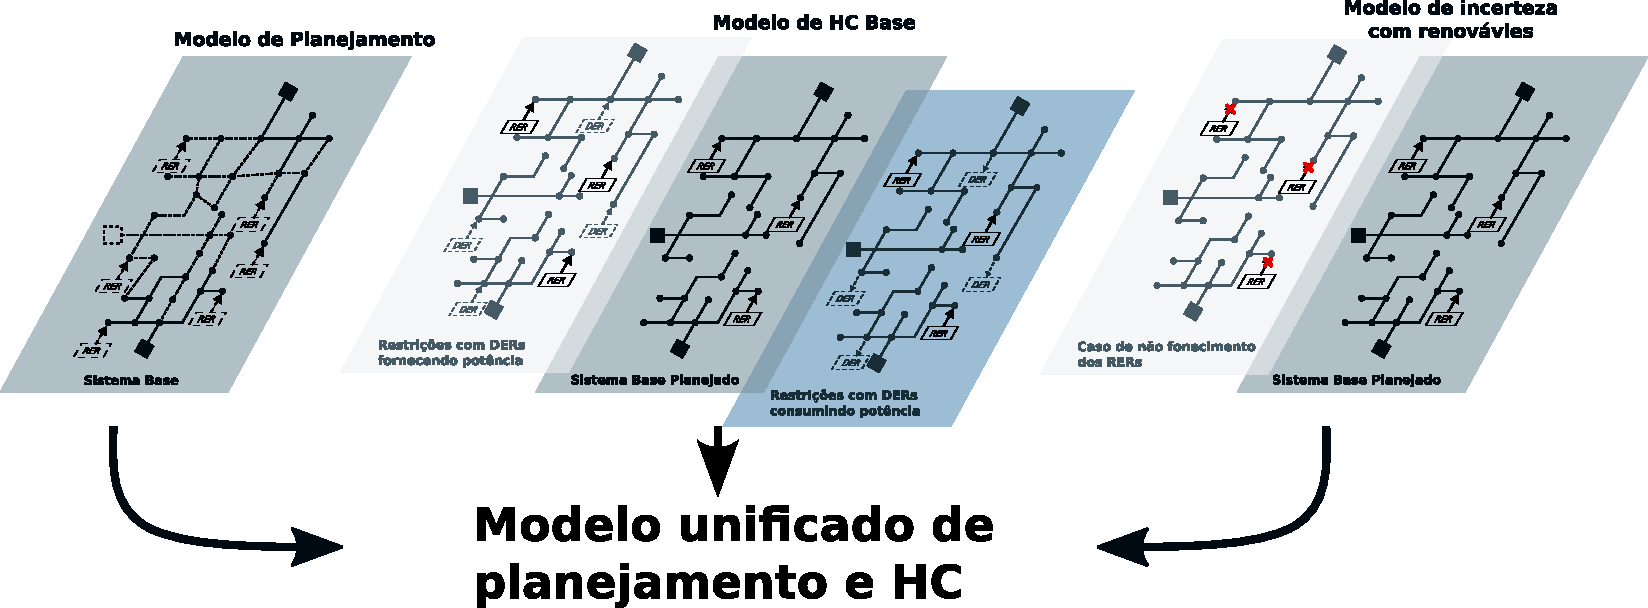
\includegraphics[width=1\textwidth]{cap3/modelo-new.pdf}\\
    Fonte: Próprio autor
    \label{fig:model_hc}
\end{figure}

Optou-se por avaliar o valor do \ac{HC} através do menor valor de injeções de corrente dos recursos energéticos distribuídos em cada estágio. Observa-se que esta proposição assume que cada estágio terá seu valor de \ac{HC}, porém, através da adição de novas restrições, impõe-se que a injeção de corrente deve no mínimo se manter igual durante a evolução dos estágios. 

Não é considerado um \ac{HC} dinâmico, devido ao autor deste trabalho compreender que esta avaliação é melhor feita durante o planejamento da operação, fugindo do escopo do \ac{PESD}. Por fim, considera-se que há um recurso energético distribuído em todos os barramentos do sistema de distribuição que possuem carga, porém, estes recursos só existem nas novas restrições adicionadas.

Também não é considerado o comportamento estocástico de recursos energéticos renováveis assumindo que, durante o \ac{PESD}, a empresa distribuidora não tem conhecimento do tipo de recurso que será instalado. Esta proposição segue a mesma linha de considerar que a empresa distribuidora deve ser responsável por manter o sistema de distribuição operando com qualidade, não importando quais recursos e cargas estão instalados em seu sistema de distribuição. Por outro lado, esta consideração torna a estimativa do valor de  \ac{HC} bastante conservadora, abrindo diversas oportunidades de estudos de melhoria do \ac{HC} via planejamento da operação.

Por outro lado, são considerados cenários de \ac{HC}, nos quais, podem-se simular cenários onde a análise é feita apenas para geradores distribuídos, apenas para carregamento de veículos elétricos, ou para ambos (na forma de armazenadores de energia). Estes cenários são configurados pelo parâmetro $\alpha^{HC}_u$, no qual valores positivos são considerados como geração e negativos como carga.

Desta forma, a seguir são detalhadas as alterações e adições realizadas no modelo base do problema de \ac{PESD} para incluir a estimativa do valor de \ac{HC}.

\subsection{Função objetivo para capacidade de acomodação}

Conforme discutido na revisão bibliográfica, o valor de \ac{HC}  é definido como a máxima injeção possível de recursos energéticos distribuídos no sistema de distribuição. Porém, podemos considerar também um \ac{HC} local, como a máxima injeção possível de recursos energéticos em um nó do sistema de distribuição. De toda forma, foi escolhido neste modelo que todos os nós do sistema injetam a mesma quantidade de corrente ($J^{HC}_t$) no estágio $t$ e que o valor de \ac{HC} no estágio $t$ é a maximização deste valor. O valor de $J^{HC}_t$ também pode ser interpretado como a máxima corrente segura que pode ser injetada em qualquer um dos nós do sistema de distribuição. O indicador escolhido para o \ac{HC} para todos os estágios é a soma da injeção dos nós, conforme descrito em \eqref{eq:fobj_hc}. 
\begin{equation}
    \text{max.    } \sum_{t \in T} J^{HC}_t
    \label{eq:fobj_hc}
\end{equation}

Observe que este indicador é conservador  e deve ser interpretado como uma estimação da capacidade de acomodação dos nós do sistema de distribuição. Desta forma, após a decisão de quais investimentos serão realizados, novos estudos mais detalhados devem ser conduzidos a fim de obter um valor mais aproximado da realidade.


\subsection{Espelhamento do sistema de distribuição}

O espelhado do sistema de distribuição para "simular" os impactos do sistema de distribuição é realizado através da inclusão de novas restrições do comportamento do sistema. De \eqref{eq:lim_tensao_hc} até \eqref{eq:lim_dg_hc} são formulados, respectivamente, os limites operacionais das tensões, ampacidade de linhas, injeção de transformadores e de geradores distribuídos instalados na presença dos novos geradores distribuídos.
 \begin{align}
    \underline{V} \leq v_{stbhu}^{HC} \leq \overline{V}; \nonumber\\  \forall s \in \Omega^N, \forall t \in T, \forall b \in B, \forall h \in h, \forall u \in U
    \label{eq:lim_tensao_hc}\\
   f^{l, HC}_{srktbhu} \leq y^l_{srkt} \overline{F}^l_k;  \nonumber\\ \forall l \in L, \forall r \in \Omega^N, \forall s \in \Omega^{l}_r, \forall k \in K^{l}, \forall t \in T, \forall b \in B, \forall h \in h, \forall u \in U
   \label{eq:amp_hc}\\
   g^{tr, HC}_{sktbhu} \leq y^{tr}_{skt} \overline{G}^{tr}_k;  \nonumber\\ \forall tr \in TR, \forall b \in B, \forall t \in T,  \forall s \in \Omega^{N}, \forall k \in K^{tr}, \forall h \in h, \forall u \in U 
   \label{eq:ijec_hc}\\
   g^{DG,HC}_{psktbhu} \leq y^{DG}_{pskt}\overline{G}^{DG}_{pk};  \nonumber\\ \forall p \in D, \forall s \in \Omega^{DG}_p, \forall k \in K^{DG}_p, \forall t \in T, \forall b \in B, \forall h \in h, \forall u \in U\\
   g^{DG,HC}_{psktbhu} = g^{DG}_{psktbh}; \nonumber\\ \forall p \in RW, \forall s \in \Omega^{DG}_p, \forall k \in K^{DG}_p, \forall t \in T, \forall b \in B, \forall h \in h, \forall u \in U
   \label{eq:lim_dg_hc}
\end{align}

De \eqref{eq:corrent_balanc_hc} a \eqref{eq:tensao2_hc} é descrito o comportamento do sistema de distribuição na presença dos novos geradores distribuídos. Observe que em \eqref{eq:corrent_balanc_hc} a penetração dos novos recursos energéticos é adicionada como uma nova fonte de geração no barramento, impactando o fluxo de corrente nos ramos e, por sequência, nas tensões do sistema de distribuição formulado em \eqref{eq:tensao1_hc} e \eqref{eq:tensao2_hc}.
\begin{align}
    \sum_{l \in L}\sum_{k \in K^{l}} \sum_{r \in \Omega^l_s} (f^{l, HC}_{srktbhu} - f^{l, HC}_{rsktbhu}) = \alpha^{HC}_u g_{st}^{HC} + 
    \sum_{tr \in TR} \sum_{k \in K^{tr}} g^{tr, HC}_{sktbhu} \nonumber \\ + \sum_{p \in P}\sum_{k\in K^{DG}_p} g^{DG, HC}_{psktbhu} - \mu_bD_{st}; \nonumber\\
    \forall s \in \Omega^N, \forall t \in T, \forall b \in B, \forall h \in H, \forall u \in U
    \label{eq:corrent_balanc_hc}
\end{align}
\begin{align}
&- Z^l_{k}\ell_{sr}f^{l, HC}_{srktbhu} + (v_{stbhu}^{HC} - v_{rtbhu}^{HC}) \leq  M(1 - y^l_{srkt}); \nonumber\\
&\forall l \in L, \forall r \in \Omega^N, \forall s \in \Omega^{l}_r, \forall k \in K^{l}, \forall t \in T, \forall b \in B, \forall h \in H, \forall u \in U
 \label{eq:tensao1_hc}\\
&Z^l_{k}\ell_{sr}f^{l, HC}_{srktbhu} - (v_{stbhu}^{HC} - v_{rtbhu}^{HC}) \leq  M(1 - y^l_{srkt}); \nonumber\\
&\forall l \in L, \forall r \in \Omega^N, \forall s \in \Omega^{l}_r, \forall k \in K^{l}, \forall t \in T, \forall b \in B, \forall h \in H, \forall u \in U
\label{eq:tensao2_hc}
\end{align}

Por fim, a restrição \eqref{eq:volt_sub_hc} descreve o comportamento das tensões nos barramentos de subestação. Em \eqref{eq:hc_load} define que a corrente injetada deve ser a mesma em todos os nós. Em \eqref{eq:hc_no_sub} não permite a injeção de novos recursos distribuídos em barramentos sem cargas. Já em \eqref{eq:mantem_gera_tpcco_hc} garante que a injeção de corrente dos novos recursos seja no mínimo a mesma durante a evolução do \ac{PESD}.
\begin{align}
&v_{stbhu}^{HC} = V^{SS} \sum_{tr \in TR}\sum_{k \in K^{tr}} y^{tr}_{skt} ; \; \; \forall s \in \Omega^{SS}, \forall t \in T, \forall b \in B, \forall h \in H, \forall u \in U
\label{eq:volt_sub_hc}\\
&g^{HC}_{st} = J^{HC}_t;\; \; \forall t \in T, \forall s \in   \Omega^{LN}_t\label{eq:hc_load}\\
&g^{HC}_{st} = 0;\; \; \forall t \in T, \forall s \in   \Omega^{N}\setminus \Omega^{LN}_t\label{eq:hc_no_sub}\\
&J^{HC}_{t} \leq J^{HC}_{{t+1}}; \; \; \forall t \in \{1, 2, ..., n_{T} -1 \}
\label{eq:mantem_gera_tpcco_hc}
\end{align}

\vspace{-0.25cm}
\subsection{Restrições de domínio}

Para assegurar uma melhor reprodutibilidade do modelo proposto, segue de \eqref{eq:dom_corr_hc} a \eqref{eq:dom_j_hc} as restrições de domínio das variáveis adicionadas no modelo.
\begin{align}
&f^{l, HC}_{srktbhu} \geq 0; \; \;\forall l \in L, \forall s \in \Omega^N, \forall r \in \Omega^l_s, \forall k \in K^l, \forall t \in T, \forall b \in B , \forall h \in H, \forall u \in U \label{eq:dom_corr_hc}\\
&g^{DG, HC}_{sktbhu} \geq 0; \; \; \forall s \in \Omega^N, \forall k \in K^{DG}, \forall t \in T, \forall b \in B, \forall h \in H, \forall u \in U \label{eq:dom_gd_hc}\\
&g^{tr, HC}_{sktbhu} \geq 0; \; \; \forall tr \in TR, \forall s \in \Omega^N, \forall k \in K^{tr}, \forall t \in T, \forall b \in B, \forall h \in H, \forall u \in U\\
&g^{HC}_{st} \geq 0 ; \; \; \forall s \in \Omega^N, \forall t \in T \label{eq:dom_g_hc}\\
&J^{HC}_{t} \geq 0 ; \; \; \forall t \in T \label{eq:dom_j_hc}
\end{align}

\subsection{Limitações do modelo proposto}

Como o modelo base, o modelo proposto é linear inteiro-misto multiobjetivo, portanto, as mesmas limitações aplicadas ao modelo base aplicam-se a este. Do ponto de vista da estimativa do \ac{HC}, este modelo apresenta uma estimativa conservadora, tanto por assumir o não conhecimento dos geradores distribuídos que podem ser instalados, quanto por buscar maximizar o valor de \ac{HC} via injeção de corrente, dado que a potência depende tanto do valor da corrente, quanto do valor da tensão em cada barramento.

Outra limitação do modelo é considerar a mesma corrente simulada em todos os nós para estimar o \ac{HC}. Este fator, 
torna o modelo ainda mais conservador e não considera outros fatores como \ac{HC} locais diferentes para cada nó, nem leva em consideração outros indicadores de \ac{HC}. Entretanto, este modelo consegue integrar o \ac{PESD} com uma estimativa do \ac{HC}, o que, até o momento, não foram encontradas propostas semelhantes na literatura acadêmica. 

A seguir são demonstrados resultados numéricos dos modelos apresentados.
